\subsection{Dati e risultati}

\begin{figure*}[t]
    \centering
    \begin{circuitikz}[x=0.9cm, y=0.9cm]
        \foreach \i in {1,...,4} {
            \draw (\i*3.8, 0) -- (\i*3.8, 3) -- (\i*3.8 + 2, 3) -- (\i*3.8 + 2, 0) -- (\i*3.8, 0);
            \draw (\i*3.8, 2.25) node[right] (J\i) {J\i};
            \draw (\i*3.8, 0.75) node[right] (K\i) {K\i};
            \draw (\i*3.8 + 2, 2.25) node[left] (Q\i) {Q\i};
            \draw (\i*3.8 + 2, 0.75) node[left] {$\overline{\text{Q\i}}$};
            \draw (\i*3.8 + 1, 3) node[anchor=north] (PR\i) {PR};
            \draw (\i*3.8 + 1, 0) node[anchor=south] (CL\i) {CL};
            \draw (\i*3.8, 1.25) -- (\i*3.8 + 0.25, 1.5) -- (\i*3.8, 1.75);
            \coordinate (CLK\i) at (\i*3.8, 1.5);
            \coordinate (preCLK\i) at (\i*3.8 - 0.5, 1.5);
            \coordinate (preK\i) at (\i*3.8 - 0.2, 0.75);
        };
        \coordinate (init) at (1, -1);
        \draw
            (1, -2) node[rground] {}
            to [C, l=470 nF] (init) node[left] {A}
        ;
        \draw
            (init) to [R, l=10<\kilo\ohm>] (1, 1)
            node[anchor=south] {$V\ped{CC}$}
        ;
        \draw
            (init) -| (2.5, 4) -| (PR1)
            (init) -| (CL2)
            (init) -| (CL3)
            (init) -| (CL4)
            
            (Q1) -| (J2.west)
            (Q1) --++ (1, 0) --++ (0, 4.5) node[above] {Q1}
            (Q1) --++ (1, 0) |- (preK2) ++ (0.1, 0) circle (0.1cm)
            
            (Q2) -| (J3.west)
            (Q2) --++ (1, 0) --++ (0, 4.5) node[above] {Q2}
            (Q2) --++ (1, 0) |- (preK3) ++ (0.1, 0) circle (0.1cm)
            
            (Q3) -| (J4.west)
            (Q3) --++ (1, 0) --++ (0, 4.5) node[above] {Q3}
            (Q3) --++ (1, 0) |- (preK4) ++ (0.1, 0) circle (0.1cm)
            
            (Q4.east) --++ (0.5, 0) |- (3, 6) |- (J1.west)
            (Q4.east) --++ (1, 0) --++ (0, 4.5) node[above] {Q4}
            (3, 6) |- (preK1) ++ (0.1, 0) circle (0.1cm)
        ;
        \draw
            (1, 4.75) node[left] (CLK) {CLK}
            (CLK) -| (preCLK1) -- (CLK1)
            (CLK) -| (preCLK2) -- (CLK2)
            (CLK) -| (preCLK3) -- (CLK3)
            (CLK) -| (preCLK4) -- (CLK4)
        ;
        \draw
            (CL1.south) ++ (0, -0.1) circle (0.1) ++ (0, -0.1) --++ (0, -0.5) node[right] {$V\ped{CC}$}
            (PR2.north) ++ (0, 0.1) circle (0.1) ++ (0, 0.1) --++ (0, 0.75) node[above] {$V\ped{CC}$}
            (PR3.north) ++ (0, 0.1) circle (0.1) ++ (0, 0.1) --++ (0, 0.75) node[above] {$V\ped{CC}$}
            (PR4.north) ++ (0, 0.1) circle (0.1) ++ (0, 0.1) --++ (0, 0.75) node[above] {$V\ped{CC}$}
        ;
    \end{circuitikz}
    \caption{Shift resister ciclico.}
    \label{fig:shift12}
\end{figure*}

\paragraph{Shift register.}

Gli shift register, o registri a scorrimento, sono circuiti che mantengono in memoria un certo numero di bit
e spostano la sequenza di 1 bit ogni volta che arriva un fronte d'onda positivo al clock
(I FF da noi usati erano positive edge triggered).
I registri a scorrimento
servono principalmente per costruire convertitori seriale-parallelo e parallelo-seriale, ma trovano
impiego anche in altri campi.


La figura \ref{fig:shift12} mostra lo shift register che abbiamo costruito. Il registro
è costruito con 4 flip-flop JK e di conseguenza memorizza 4 bit. Inoltre l'uscita dell'ultimo FF
è collegata con l'entrata del primo, per fare un registro ciclico, che cicla la sequenza di bit.

Vediamo come funziona il circuito. La prima cosa da fare all'accensione del circuito è caricare
una sequenza di bit in memoria. Questo risultato è ottenuto grazie alle porte preser (PR) e clear (CL),
che, come fa intuire il nome, servono rispettivamente per importare un valore all'uscita Q o a
``pulire'' i valori precedenti, impostando 0. Entrambe queste entrate sono negate, cioè vengono impostate
a 1 se non si vuole usarle. Infatti le porte preset dei FF 2, 3 e 4 e la clear del primo sono
state collegate tutte a $V\ped{CC}$, in modo che non siano mai utilizzate. Il trucco viene poi con
la resistenza e il condensatore; il punto A è collegato con il preset del primo FF
e ai clear dei restanti. All'accensione dell'alimentazione il condensatore impiega un certo
tempo per caricarsi, per cui all'inizio il punto A è a 0 logico e carica un 1 sul primo FF,
mentre gli altri sono impostati a 0 mediante le porte clear. Quando il condensatore si carica,
A diventa un 1 logico e fa si che tutti i preset e clear siano disattivati.

Ogni volta che arriva un fronte d'onda positivo nel clock,
i flip-flop leggono i loro ingressi e copiano il valore all'uscita. Poiché ci sono
dei ritardi di pochi nanosecondi tra l'arrivo del fronte e la copiatura del valore in ingresso,
si ha che la sequenza di bit viene spostata a destra (si noti che l'ultimo valore $Q_4$ viene spostato
a $Q_1$).

Abbiamo quindi collegato il circuito alla schedina con i LED che ci permette di visualizzare i valori
0 o 1 alle uscite $Q_1,\dots,Q_4$. Fornendo un onda quadra di frequenza bassa (1-10 Hz) è stato possibile
vedere il bit 1 impostato all'inizio ciclare.

\paragraph{Contatore a 8 bit.}

Un utilissima applicazione dei FF sono i contatori. A parte il loro utilizzo in moltissime componenti
elettroniche, in ambito scientifico sperimentale sono molto utili per realizzare esperimenti
in cui sia necessario contare degli oggetti, per esempio il numero di particelle arrivate su di un rivelatore.
In queste applicazioni si usano degli integrati come il 74LS191, che includono al loro interno tutto il necessario
per il conteggio. Non resta che collegarli opportunamente.

Tuttavia i 74LS191 sono contatori a 4 bit e noi vogliamo realizzare un contatore a 8 bit, per
cui ce ne servono 2 in cascata, il secondo dei quali conta il numero delle volte che il primo
è andato in overflow/underflow. Il circuito in figura \ref{fig:contatore12} è il circuito adatto allo scopo.

Gli integrati 74LS191 hanno le seguenti porte:

\begin{itemize}
    \item{CE (Count Enable): se bassa il contatore è abilitato, altrimenti il contatore non fa nulla.}
    \item{D/$\overline{\text{U}}$ (Down/Up): se 0 il contatore conta da 0 (0000) a 15 (1111), mentre se
        è alta il conteggio avviene al rovescio.}
    \item{RC (Ripple Clock): quest'uscita è normalmente a 1, ma scende a 0 quando si è raggiunto il valore massimo
        o minimo, in base alla direzione in cui si sta contando (crescente o decrescente rispettivamente).
        Rimane bassa finché il clock non ritorna basso (il 74LS191 è positive edge triggered).}
    \item{LOAD e $P_1,\dots,P_4$: Quando LOAD è basso il segnale agli ingressi $P_1,\dots,P_4$ viene copiato
        in modo asincrono alle uscite, indipendentemente dal clock. Utile per impostare i valori iniziali.}
\end{itemize}

La parte in basso a sinistra del circuito è composta da un interruttore che permette di scegliere la direzione
del conteggio. Il FF JK serve per assicurarsi che lo stato delle porte U/$\overline{\text{U}}$ venga cambiato
soltanto quando il clock è alto, poiché sulle specifiche del 74LS191 è scritto che cambiarlo in altri momenti
causa uno stato non definito all'interno dell'integrato. Il flip-flop cambia lo stato di Q e quindi delle porte
U/$\overline{\text{U}}$ soltanto quando il clock diventa alto, poiché i JK sono positive edge triggered.
La resistenza da \SI{1}{\kilo\ohm} è un semplice pull-down.

In seguito sono presenti due contatori a 4 bit, collegati a clock e al FF JK come visto prima. Inolte
la porta CE (Count Enable) del primo è collegata al riferimento per attivare il contatore, mentre quella del
secondo è collegata all'uscita RC del primo, in modo che il secondo venga attivato solo quando il primo
va in overflow/undeflow. Inoltre è necessario azzerare il contatore all'accensione. Questo viene assicurato
collegando a comune le uscite $P_1,\dots,P_4$ di ciascun contatore e collegando la porta LOAD, attiva negativa,
con una resistenza ed un condensatore, come è stato fatto nel circuito precedente. All'accensione il condensatore
impiega del tempo per caricarsi e nel frattempo attiva la porta LOAD.

Quindi questo circuito conta il numero di fronti d'onda che arrivano dal clock. Se il clock è collegato
ad un rilevatore di particelle, per esempio, verrà contato il numero di particelle rilevate. Ovviamente
il rivelatore deve fornire un segnale a 5 volt quando arriva la particella.

La verifica del funzionamento è stata fatta con la solita scheda coi LED, fornendo sul clock
un onda quadra di frequenza bassa (pochi Hertz) per poter vedere il conteggio. Una verifica
migliore verrà fatta nel prossimo paragrafo.

\begin{figure*}[p]
    \centering
    \begin{circuitikz}[scale=0.8, transform shape]
        \draw
            (3, -4) -| (5, -7) -| (3, -4)
            (3, -4.75) node[right] (J) {J}
            (3, -6.25) node[right] (K) {K}
            (5, -4.75) node[left] (Q) {Q}
            (5, -6.25) node[left] {$\overline{\text{Q}}$}
            (3, -5.25) -- (3.25, -5.5) -- (3, -5.75)
            (4, -4) node[below] (PR) {PR} to[short, o-o] ++ (0, 0.5) node[above] {$V\ped{CC}$}
            (4, -7) node[above] (CL) {CL} to[short, o-o] ++ (0, -0.5) node[below] {$V\ped{CC}$}
        ;
        \coordinate (preCLK_JK) at (2, -5.5);
        \coordinate (preJ) at (2.5, -4.75);
        \coordinate (preK) at (2.5, -6.25);
        \coordinate (CLK_JK) at (3, -5.5);
        
        \draw
            (-1, -6) node[above] {$V\ped{CC}$} |- (0, -7) ++ (0.1, 0) circle (0.1)
            ++ (0.1, 0) --++ (0.5, 0.3) ++ (0, -0.3) circle (0.1) ++ (0.1, 0)
            coordinate (switch)
        ;
        
        \draw
            (switch) -| (preJ) -- (J.west)
            (switch) -| (preK) to [short, -o] (K.west)
            (switch) --++ (0.5, 0) to[R, l=1<\kilo\ohm>] ++(0, -1.5) node[rground] {}
        ;
    
        \draw
            (-1, 0) node[left] (CLK) {CLK} -| (preCLK_JK) -- (CLK_JK)
        ;
        
        \foreach \i in {0,1} {
            \draw (11, -\i*6 + 2) -| (14, -\i*6 - 3) -| (11, -\i*6 + 2);
            \draw
                (11, -\i*6 + 2 - 0.5) node[right] (P0\i) {P0}
                (11, -\i*6 + 2 - 1) node[right] (P1\i) {P1}
                (11, -\i*6 + 2 - 1.5) node[right] (P2\i) {P2}
                (11, -\i*6 + 2 - 2) node[right] (P3\i) {P3}
                (11, -\i*6 + 2 - 3.5) node[right] (CE\i) {CE}
                (11, -\i*6 + 2 - 4) node[right] (DU\i) {D/$\overline{\text{U}}$}
                (11, -\i*6 + 2 - 4.5) node[right] (LOAD\i) {LOAD}
                (11, -\i*6 + 2 - 2.5) --++ (0.25, -0.25) --++ (-0.25, -0.25)
                (14, -\i*6 + 2 - 0.5) node[left] (Q0\i) {Q0}
                (14, -\i*6 + 2 - 1) node[left] (Q1\i) {Q1}
                (14, -\i*6 + 2 - 1.5) node[left] (Q2\i) {Q2}
                (14, -\i*6 + 2 - 2) node[left] (Q3\i) {Q3}
                (14, -\i*6 + 2 - 3.5) node[left] (CR\i) {RC}
            ;
            \draw
                (P0\i) --++ (-1, 0)
                (P1\i) --++ (-1, 0)
                (P2\i) --++ (-1, 0)
                (P3\i) --++ (-1, 0) |- ++ (-1, 2) node[rground] {}
                (Q0\i.east) to[short, -o]++ (1, 0)
                (Q1\i.east) to[short, -o]++ (1, 0)
                (Q2\i.east) to[short, -o]++ (1, 0)
                (Q3\i.east) to[short, -o]++ (1, 0)
            ;
            \coordinate (CLK\i) at (11, -\i*6 + 2 - 2.75);
            \coordinate (preCE\i) at (10.5, -\i*6 + 2 - 3.5);
        };

        \draw
            (Q) --++ (2, 0) |- (DU0.west)
            (Q) ++ (2, 0) |- (DU1.west)
            (CLK) --++ (7, 0) |- (CLK0)
            (CLK) ++ (7, 0) |- (CLK1)
            (CR0.east)  to[short, o-] ++ (1, 0) |- ++ (-6.5, -2) |- (preCE1) to[short, -o] (CE1.west)
            (CE0.west) to[short, o-] ++ (-1, 0) node[rground] {}
        ;
        \draw
            (LOAD0.west) to[short, o-] ++(-0.1, 0) -| (7.5, -8.5)
            (LOAD1.west) to[short, o-] ++(-0.1, 0) -| (7.5, -11)
            --++ (1, 0)
        ;
        \coordinate (LS) at (8.5, -11);
        \draw
            (LS) to[C, l=470 nF] ++ (0, -1) node[rground] {}
            (LS) to[R, l_=10<\kilo\ohm>] ++(0, 1.5) node[above] {$V\ped{CC}$}
        ;
    \end{circuitikz}
    \caption{Contatore a 8 bit.}
    \label{fig:contatore12}
\end{figure*}

\begin{figure*}
    \centering
    \begin{circuitikz}[scale=0.7, transform shape]
       \draw
           (3, -4) -| (5, -7) -| (3, -4)
           (3, -4.75) node[right] (J) {J}
           (3, -6.25) node[right] (K) {K}
           (5, -4.75) node[left] (Q) {Q}
           (5, -6.25) node[left] {$\overline{\text{Q}}$}
           (3, -5.25) -- (3.25, -5.5) -- (3, -5.75)
           (4, -4) node[below] (PR) {PR} to[short, o-o] ++ (0, 0.5) node[above] {$V\ped{CC}$}
           (4, -7) node[above] (CL) {CL} to[short, o-o] ++ (0, -0.5) node[below] {$V\ped{CC}$}
       ;
       \coordinate (preCLK_JK) at (2, -5.5);
       \coordinate (preJ) at (2.5, -4.75);
       \coordinate (preK) at (2.5, -6.25);
       \coordinate (CLK_JK) at (3, -5.5);
       
       \draw
           (-1, -6) node[above] {$V\ped{CC}$} |- (0, -7) ++ (0.1, 0) circle (0.1)
           ++ (0.1, 0) --++ (0.5, 0.3) ++ (0, -0.3) circle (0.1) ++ (0.1, 0)
           coordinate (switch)
       ;
       
       \draw
           (switch) -| (preJ) -- (J.west)
           (switch) -| (preK) to [short, -o] (K.west)
           (switch) --++ (0.5, 0) to[R, l=1<\kilo\ohm>] ++(0, -1.5) node[rground] {}
       ;
       \draw
           (-1, 0) node[left] (CLK) {CLK} -| (preCLK_JK) -- (CLK_JK)
       ;
       
       \foreach \i in {0,1} {
           \draw (11, -\i*6 + 2) -| (14, -\i*6 - 3) -| (11, -\i*6 + 2);
           \draw
               (11, -\i*6 + 2 - 0.5) node[right] (P0\i) {P0}
               (11, -\i*6 + 2 - 1) node[right] (P1\i) {P1}
               (11, -\i*6 + 2 - 1.5) node[right] (P2\i) {P2}
               (11, -\i*6 + 2 - 2) node[right] (P3\i) {P3}
               (11, -\i*6 + 2 - 3.5) node[right] (CE\i) {CE}
               (11, -\i*6 + 2 - 4) node[right] (DU\i) {D$\overline{\text{U}}$}
               (11, -\i*6 + 2 - 4.5) node[right] (LOAD\i) {LOAD}
               (11, -\i*6 + 2 - 2.5) --++ (0.25, -0.25) --++ (-0.25, -0.25)
               (14, -\i*6 + 2 - 0.5) node[left] (Q0\i) {Q0}
               (14, -\i*6 + 2 - 1) node[left] (Q1\i) {Q1}
               (14, -\i*6 + 2 - 1.5) node[left] (Q2\i) {Q2}
               (14, -\i*6 + 2 - 2) node[left] (Q3\i) {Q3}
               (14, -\i*6 + 2 - 3.5) node[left] (CR\i) {CR}
           ;
           \draw
               (P0\i) --++ (-1, 0)
               (P1\i) --++ (-1, 0)
               (P2\i) --++ (-1, 0)
               (P3\i) --++ (-1, 0) |- ++ (-1, 2) node[rground] {}
               (Q0\i.east) to[short]++ (1, 0) % node (Q0R\i)
               (Q1\i.east) to[short]++ (1, 0)
               (Q2\i.east) to[short]++ (1, 0)
               (Q3\i.east) to[short]++ (1, 0)
           ;
           \coordinate (CLK\i) at (11, -\i*6 + 2 - 2.75); }
       
       \draw
           (Q) --++ (2, 0) |- (DU0.west)
           (Q) ++ (2, 0) |- (DU1.west)
           (CLK) --++ (7, 0) |- (CLK0)
           (CLK) ++ (7, 0) |- (CLK1)
           (CR0.east)  to[short, o-] ++ (1, 0) |- ++ (-6.5, -2) |- (CE1)
           (CE0.west) --++ (-1, 0) node[rground] {}
       ;
       \draw
           (LOAD0.west) -| (7.5, -8.5)
           (LOAD1.west) -| (7.5, -11)
           --++ (1, 0)
       ;
       \coordinate (LS) at (8.5, -11);
       \draw
           (LS) to[C, l=470 nF] ++ (0, -1) node[rground] {}
           (LS) to[R, l_=10<\kilo\ohm>] ++(0, 1.5) node[above] {$V\ped{CC}$}
       ;
       
       % PARTE Matteo
       
       % linee  b1-b4
       \foreach \j/\jtext in {0/4,1/3,2/2,3/1}{
       \draw (Q\j1.east) ++(1,0) -- ++(2.5,0) node(B\jtext)[right]{B\jtext};
       }
       % linee b5-b8
       \foreach \j/\jRa/\jRb/\jtext in {0/2/0.5/8,1/1.5/1/7,2/1/1.5/6,3/0.5/2/5}{
       \draw (Q\j0.east) ++(1,0) -- ++(\jRa,0) -- ++(0,-4) -- ++(\jRb,0) node(B\jtext)[right]{B\jtext};
       % VR+ e VR- con resistenze
       \draw
           (B1) ++ (0.1,-1) node (VRP) {$V\ped{R+}$}
           (VRP) ++ (0,-0.5) node (VRM) {$V\ped{R-}$}
           (VRP.west) -- ++(-2,0) -- ++(0,-1) to[R, l_=2.2<\kilo\ohm>] ++(0, -3) node[rground] {}
           (VRM.west) -- ++(-1,0) -- ++(0,-0.5) to[R, l=2.2<\kilo\ohm>] ++(0, -3) node[rground] {}
       ;
       % disegno il rettangolo
       \draw ($(B8.west)+(0,0.5)$) rectangle ($(VRM.west)+(3,-0.5)$);
       }
       % nodi della parte destra
       \node (IOUT)  at ($(B8.west)+(3,0)$)  [left]{$I\ped{OUT}$};
       \node (IOUTN) at ($(B5.west)+(3,0)$)  [left]{$\overline{I\ped{OUT}}$};
       \node (COMP)  at ($(B1.west)+(3,0)$)  [left]{COMP};
       \node (VLC)   at ($(VRM.west)+(2.9,0)$) [left]{VLC};
       % componenti e fine
       \draw
           (VLC.east) ++(0.1, 0) -- ++(1,0) node[rground] {}
           (COMP.east) to[C,l=10 nF, -o] ++(1.5,0) node[right]{$-15V$}
           (IOUTN.east) -- ++(1,0) node[rground]{}
           (IOUT.east) -- ++(1,0) to[R,l=2<\kilo\ohm>] ++(1.5,0) -- ++(0.5,0)  node[rground]{}
           (IOUT.east) ++(0.5,0) -- ++(0,1) node[above]{$V\ped{OUT}$}
       ;
       % label=above:$s\le3$] 
    \end{circuitikz}
    \caption{Generatore di onde a dente di sega.}
    \label{fig:ds_dac12}
\end{figure*}

\paragraph{Convertitore digitale-analogico.}

L'ultima parte dell'esperienza si è svolta con l'utilizzo del DAC08 un convertitore digitale
analogico a 8 bit  (DAC sta per Digital to Analog Converter). Questo integrato prende in input 8 canali digitali
fornisce un output analogico. Abbiamo quindi collegato il DAC08 al circuito illustrato nel paragrafo precedente,
in modo da poter costruire un generatore di onde a dente di sega come quello in
figura \ref{fig:ds_dac12}. Questo è il modo in cui la gran parte dei
generatori di forme d'onda funzionano, poiché è molto semplice da implementare.

Il DAC08 ha 8 ingressi sui quali si può inviare un numero a 8 bit per la conversione.
Ovviamente questi ingressi sono stati collegati con le uscite dei contatori, come si può vedere nello
schema in figura \ref{fig:ds_dac12}.
Oltre agli ingressi il DAC08 necessita di alimentazione ai pin 13 (positiva)
e 3 (negativa) compresa tra i 9 e i 36 V (anche non simmetrici). Noi abbiamo usato $\pm \SI{15}{\volt}$. 
Questo integrato fornisce in output una corrente
sul pin $I\ped{out}$ che è proporzionale al numero binario in ingresso, e una corrente sul $\overline{I\ped{out}}$ che è il complemento
di $I\ped{out}$. Possono essere usate entrambe; nel caso in cui una non vada usata è necessario collegarla
a terra per far fluire la corrente. Nel nostro caso, il piedino $\overline{I\ped{out}}$ è stato collegato a terra.
La corrente assorbita dal pin $I\ped{out}$ rispetta la seguente formula

\begin{figure}[b!]
    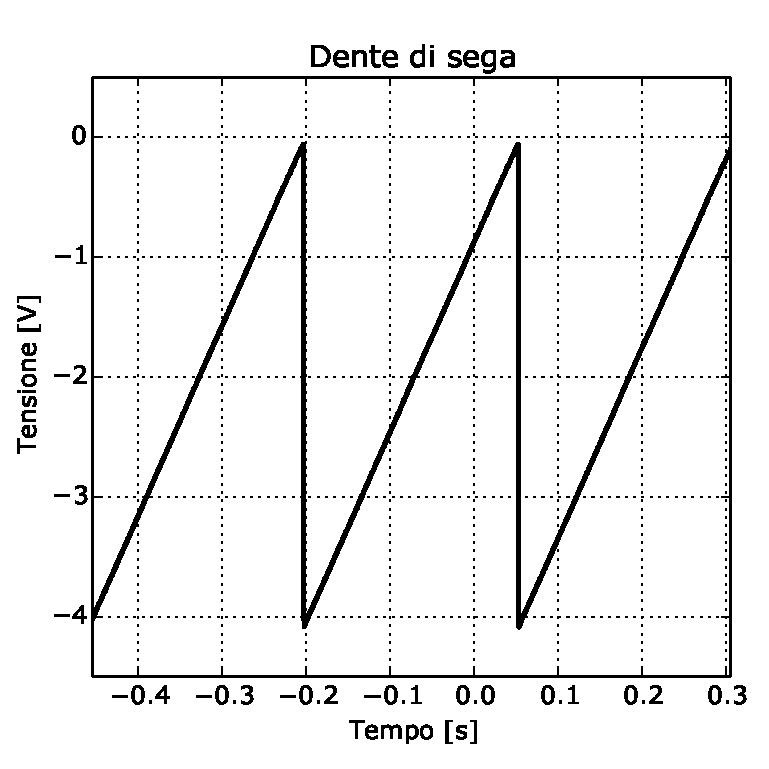
\includegraphics[width=\columnwidth]{figure/dds.pdf}
    \caption{Output del circuito \ref{fig:ds_dac12}}
    \label{fig:dds12}
\end{figure}

\begin{equation}
	I\ped{out} = I\ped{FS} \frac{n}{256} = I\ped{ref} \frac{255}{256} \cdot \frac{n}{256}
\end{equation}
%
dove $n$ è il numero binario in ingresso, $I\ped{FS} = 255/256 \times I\ped{ref}$ è la corrente massima di uscita (a $n = 255$)
e $I\ped{ref}$ è la corrente di riferimento. La corrente di riferimento può andare da 0.2 mA a 4 mA, e può essere impostata
grazie al pin VR+. Abbiamo deciso $I\ped{ref} = 2$ mA. Per ottenere questo valore è necessario sapere che
i pin VR+ e VR- sono le entrate di un operazionale. Il pin VR- è stato collegato a riferimento, mentre l'altro è stato alimentato
con 4.4 V. Interponendo tra l'alimentazione e il pin una resistenza da 2.2 \si{\kilo\ohm}, si possono generare 2 mA (l'operazionale crea un
ground virtuale). Inoltre per eliminare l'effetto delle correnti di polarizzazzione, anche VR- è stato collegato a terra con una resistenza
da 2.2 \si{\kilo\ohm}.

Poiché il circuito può essere usato con famiglie di logiche diverse dalla TTL, è necessario impostare
il tipo di logica da usare, utilizzando il pin VLC. Nel caso della TTL è sufficiente collegare il VLC a ground.
Infine il DAC08 è dotato di una porta COMP per compensare l'operazionale. Questo pin deve
essere collegato all'alimentazione negativa mediante una capacità. Abbiamo usato una capacità da 10 nF.

Infine è necessario trasformare la corrente di output in una tensione. Si è quindi collegato l'uscita a
riferimento mediante una resistenza da 2 \si{\kilo\ohm}, in modo da avere una tensione di uscita $V\ped{out}$
compresa tra 0 e -4 V (la corrente è entrante).

È chiaro che il circuito così costruito darà in output un'onda a dente di sega di frequenza dipendente da quella del clock,
o per essere più precisi pari a 1/256 della frequenza del clock. La figura \ref{fig:dds12} mostra un tipico output del circuito.
La frequenza del dente di sega in figura è 3.9 Hz, che è esattamente 1 kHz nel clock, ovvero la frequenza dell'onda quadra che abbiamo
fornito per far funzionare il circuito.
